\documentclass[10pt]{article}
\usepackage[utf8]{inputenc}
\usepackage[english]{babel}
\usepackage[font=small,labelfont=bf]{caption}
\usepackage{geometry}
\usepackage{natbib}
\usepackage{pxfonts}
\usepackage{graphicx}
\usepackage{newfloat}
\usepackage{setspace}
%\doublespacing

\newcommand{\argmax}{\mathop{\mathrm{argmax}}\limits}

\title{\textit{Supplemental Figures for}: A Gaussian process model of human electrocorticographic data} 
\author{
  Lucy L. W. Owen$^{1}$,
  Andrew C. Heusser$^{1, 2}$, and
  Jeremy R. Manning$^{1\ast}$\\\\
$^{1}$Department of Psychological and Brain Sciences, Dartmouth College,\\
Hanover, NH 03755, USA\\
$^{2}$Akili Interactive,\\
Boston, MA 02110, USA}

\bibliographystyle{apa}

\begin{document}
\maketitle

\setcounter{equation}{0}
\setcounter{figure}{0}
\setcounter{table}{0}
\setcounter{page}{1}
\setcounter{section}{0}
\makeatletter
\renewcommand{\theequation}{S\arabic{equation}}
\renewcommand{\thefigure}{S\arabic{figure}}
\renewcommand{\bibnumfmt}[1]{[S#1]}
\renewcommand{\citenumfont}[1]{S#1}


\begin{figure}[b!]
\centering
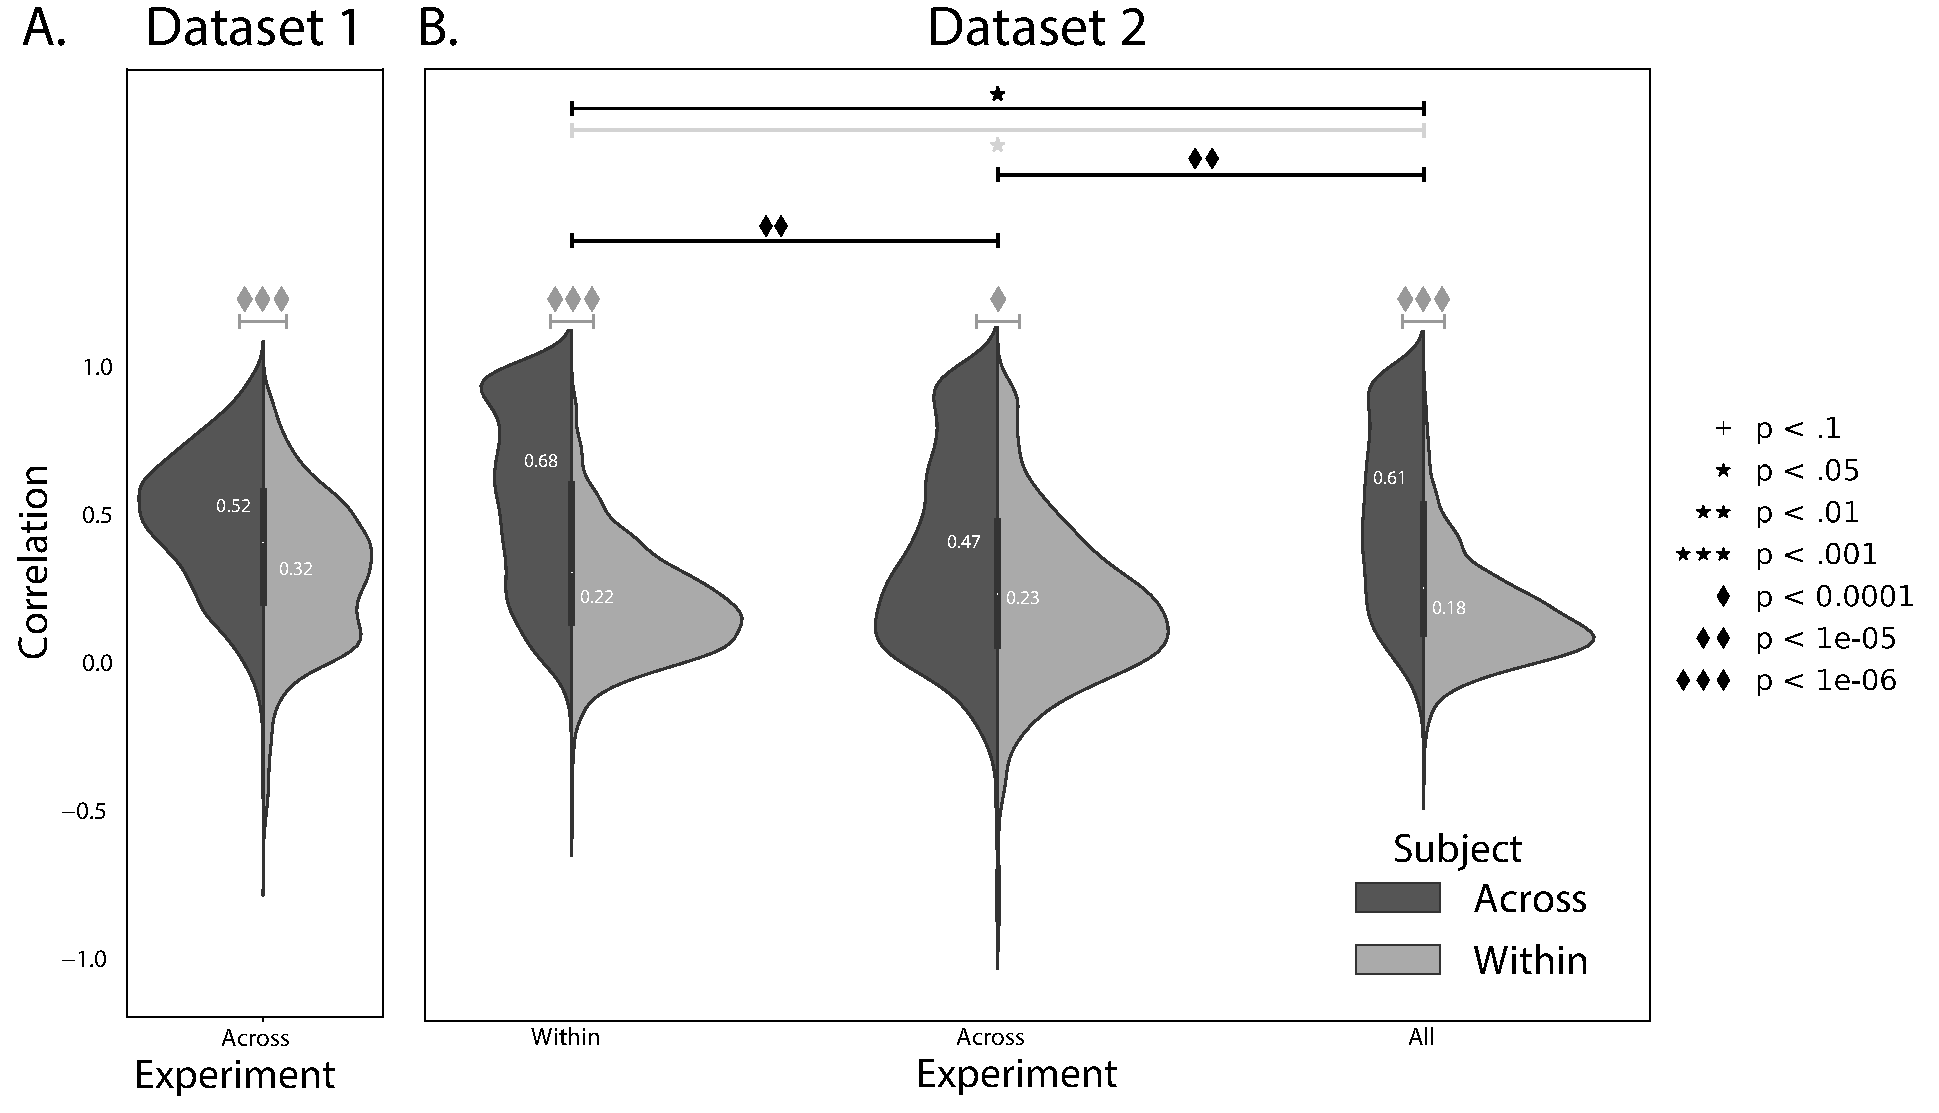
\includegraphics[width=0.6\textwidth]{figs/supplemental_1}
\caption{\textbf{Reconstruction quality for datasets 1 and 2.}
  \textbf{A. Distributions of correlations between observed versus
    reconstructed activity by electrode, for Dataset 1.} The split violin
  plot reflects the same data as Figure~3A, presented here for
  comparison.  The ``\textbf{B. Distributions of correlation between
    observed versus reconstructed activity by electrode, for Dataset
    1.}  The right-most split violin plot (``All'') reflects the same data as Figure~3B,
  presented here for comparison.  The ``Within'' plot reflects the
  same analyses, but limited to models that were trained and tested on
  the same Dataset 2 experiments.  The ``Across'' plot reflects the
  same analyses, but limited to models that were trained and tested on
  \textit{different} Dataset 2 experiments.  All plots: the dark gray
  distributions denote across-subject correlations (model trained on
  all but one patient and tested on the held-out patient), and the
  light gray distributions denote within-subject correlations (model
  trained on all but one electrode from one patient, and tested on the
  held-out electrode).  The horizontal bars denote $t$-tests between
  the corresponding distributions, and the white numbers reflect the
  distribution means.  The symbols denote the corresponding $p$-values
of those statistical tests.}
\label{fig:supplemental_1}
\end{figure}


\begin{figure}[p]
\centering
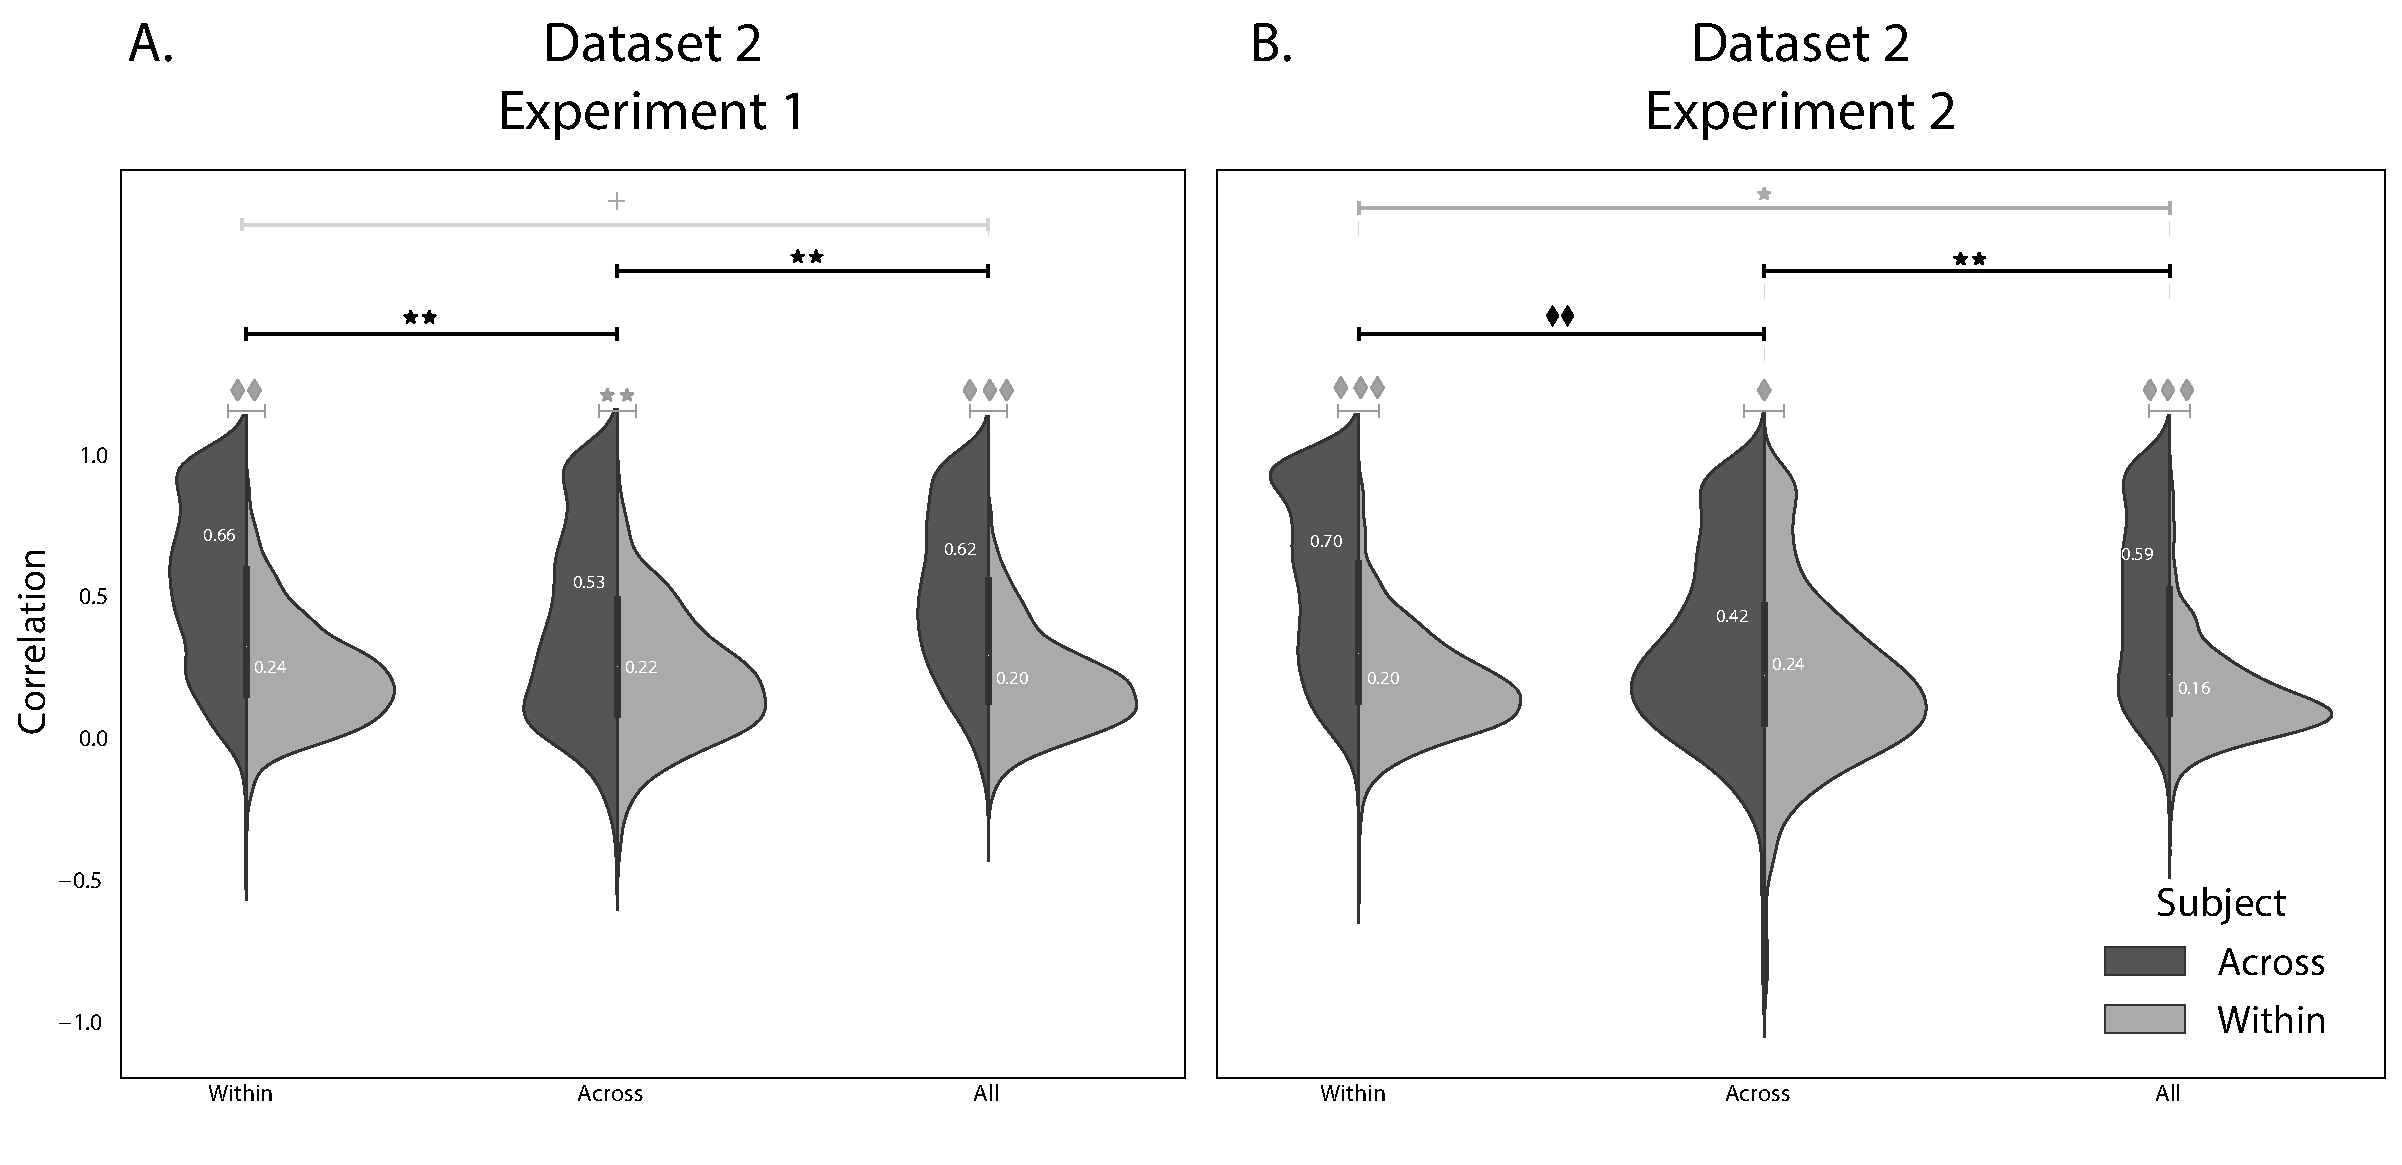
\includegraphics[width=\textwidth]{figs/supplemental_2}
\caption{\textbf{Reconstruction quality for Dataset 2,
    Experiments 1 and 2.} \textbf{A. Distributions of correlations
    between observed versus reconstructed activity by electrode, for
    Experiment 1.}  Each split violin plot and horizontal bar is in
  the same format as the plots in Figure~\ref{fig:supplemental_1}.
  ``Within'' denotes within-subject correlations (model trained on all
  but one electrode from one patient, and tested on the held-out
  electrode); ``Across'' denotes across-subject correlations (model
  trained an all but one patient and tested on the held-out patient);
  ``All'' denotes a model trained on all data from all patients,
  except for one held-out electrode (and tested on the held-out
  electrode).  \textbf{B. Distributions of correlations between
    observed versus reconstructed activity by electrode, for
    Experiment 2.}  All of the plots and bars are in the same format
  as those in Panel A.}
\label{fig:supplemental_2}
\end{figure}

\begin{figure}[p]
\centering
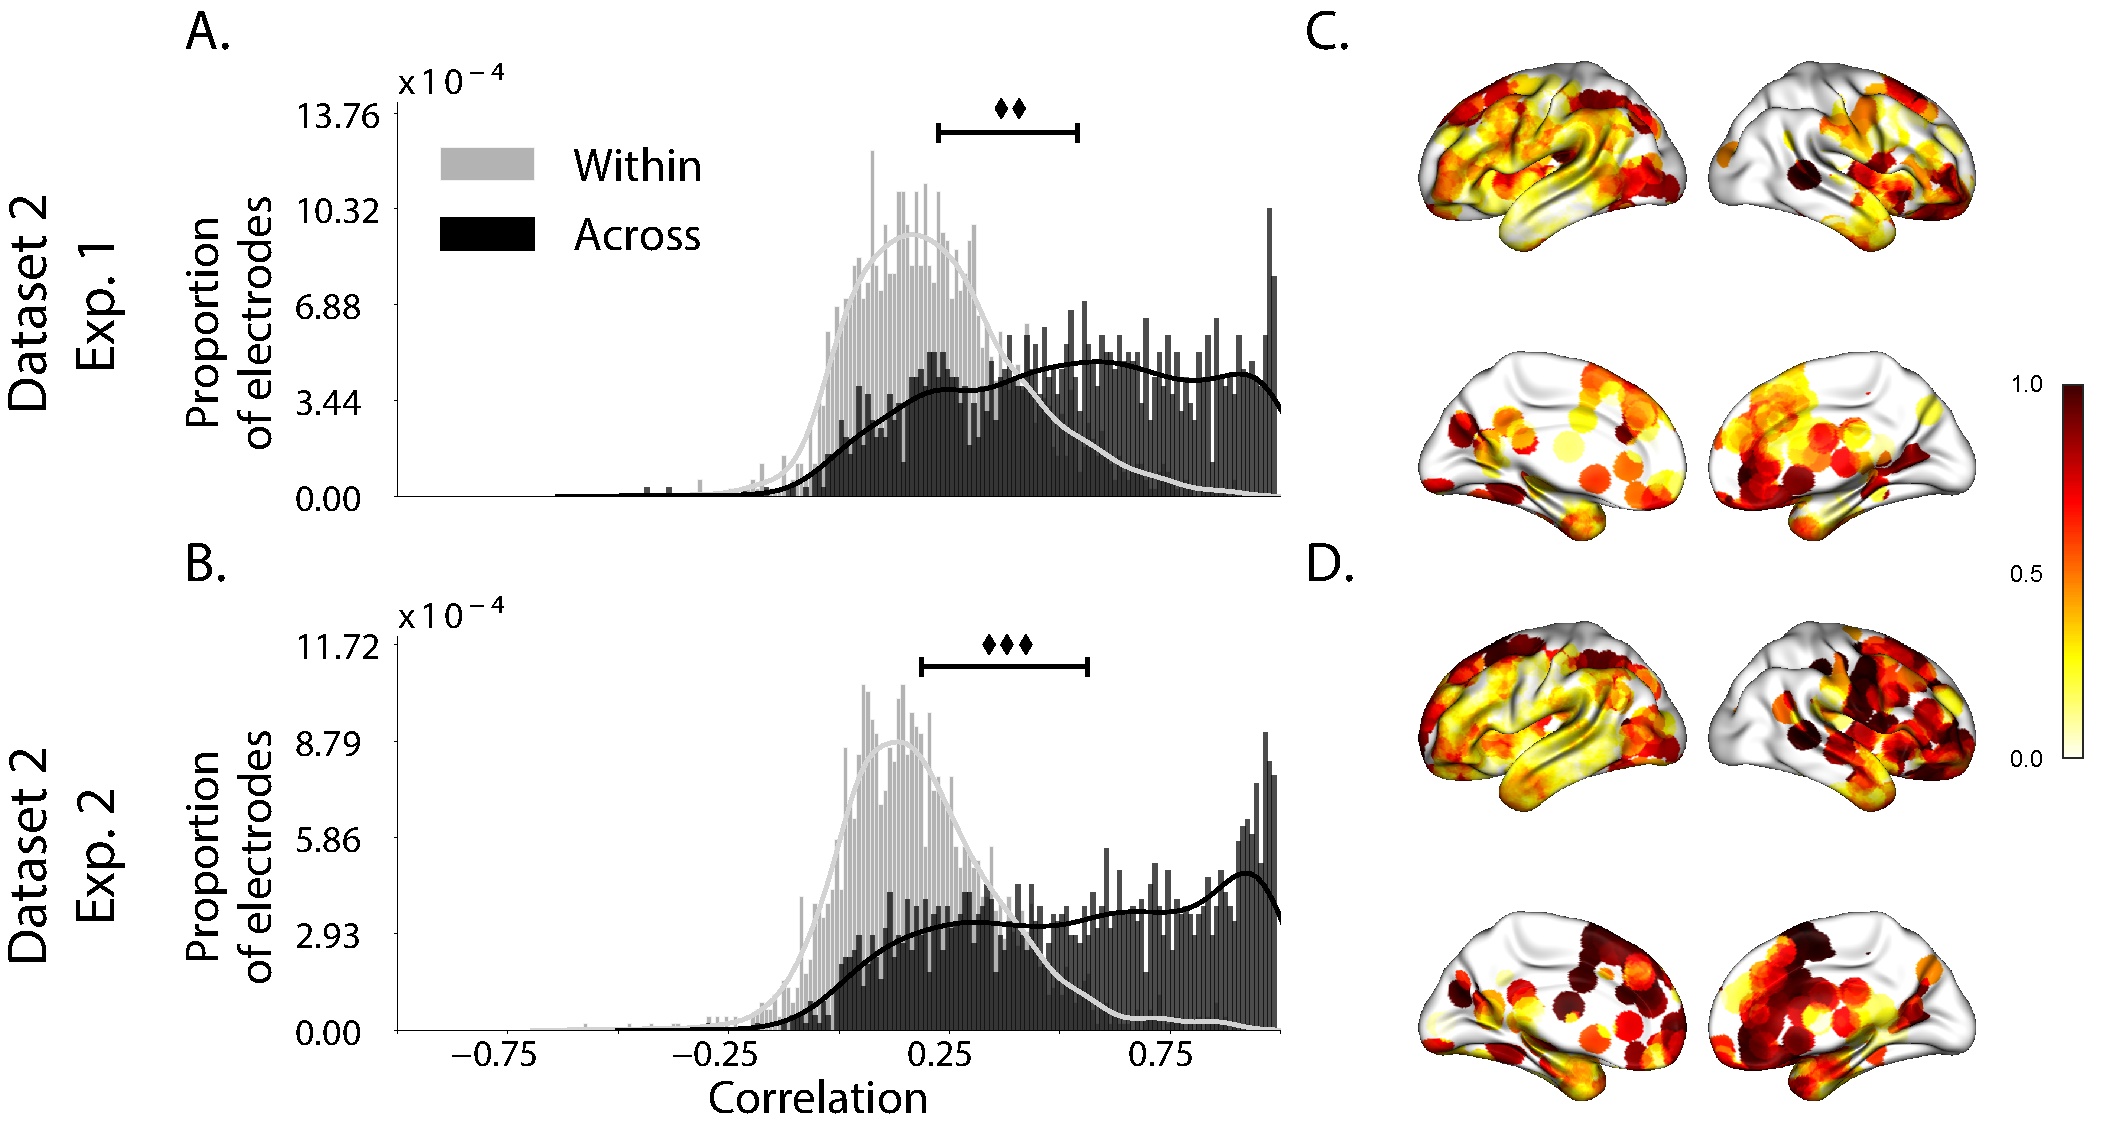
\includegraphics[width=\textwidth]{figs/supplemental_3}
\caption{\textbf{Reconstruction quality for each experiment.} \textbf{A. \& C.  Distributions
      of correlation coefficients.}  Across all electrodes from all
    patients in the labeled experiment from dataset 2, the panel displays the distribution of correlations between the observed and reconstructed LFP data using models trained on data from all other patients (Across, in black) and all other electrodes from the same patient (Within, in gray). 
    \textbf{B. \& D. Correlation maps.}  The glass brain maps display the
    average correlation between the observed LFP data and the across-subjects model reconstructed data by location, for each labeled experiment.}
\label{fig:supplemental_3}
\end{figure}


\begin{figure}[p]
\centering
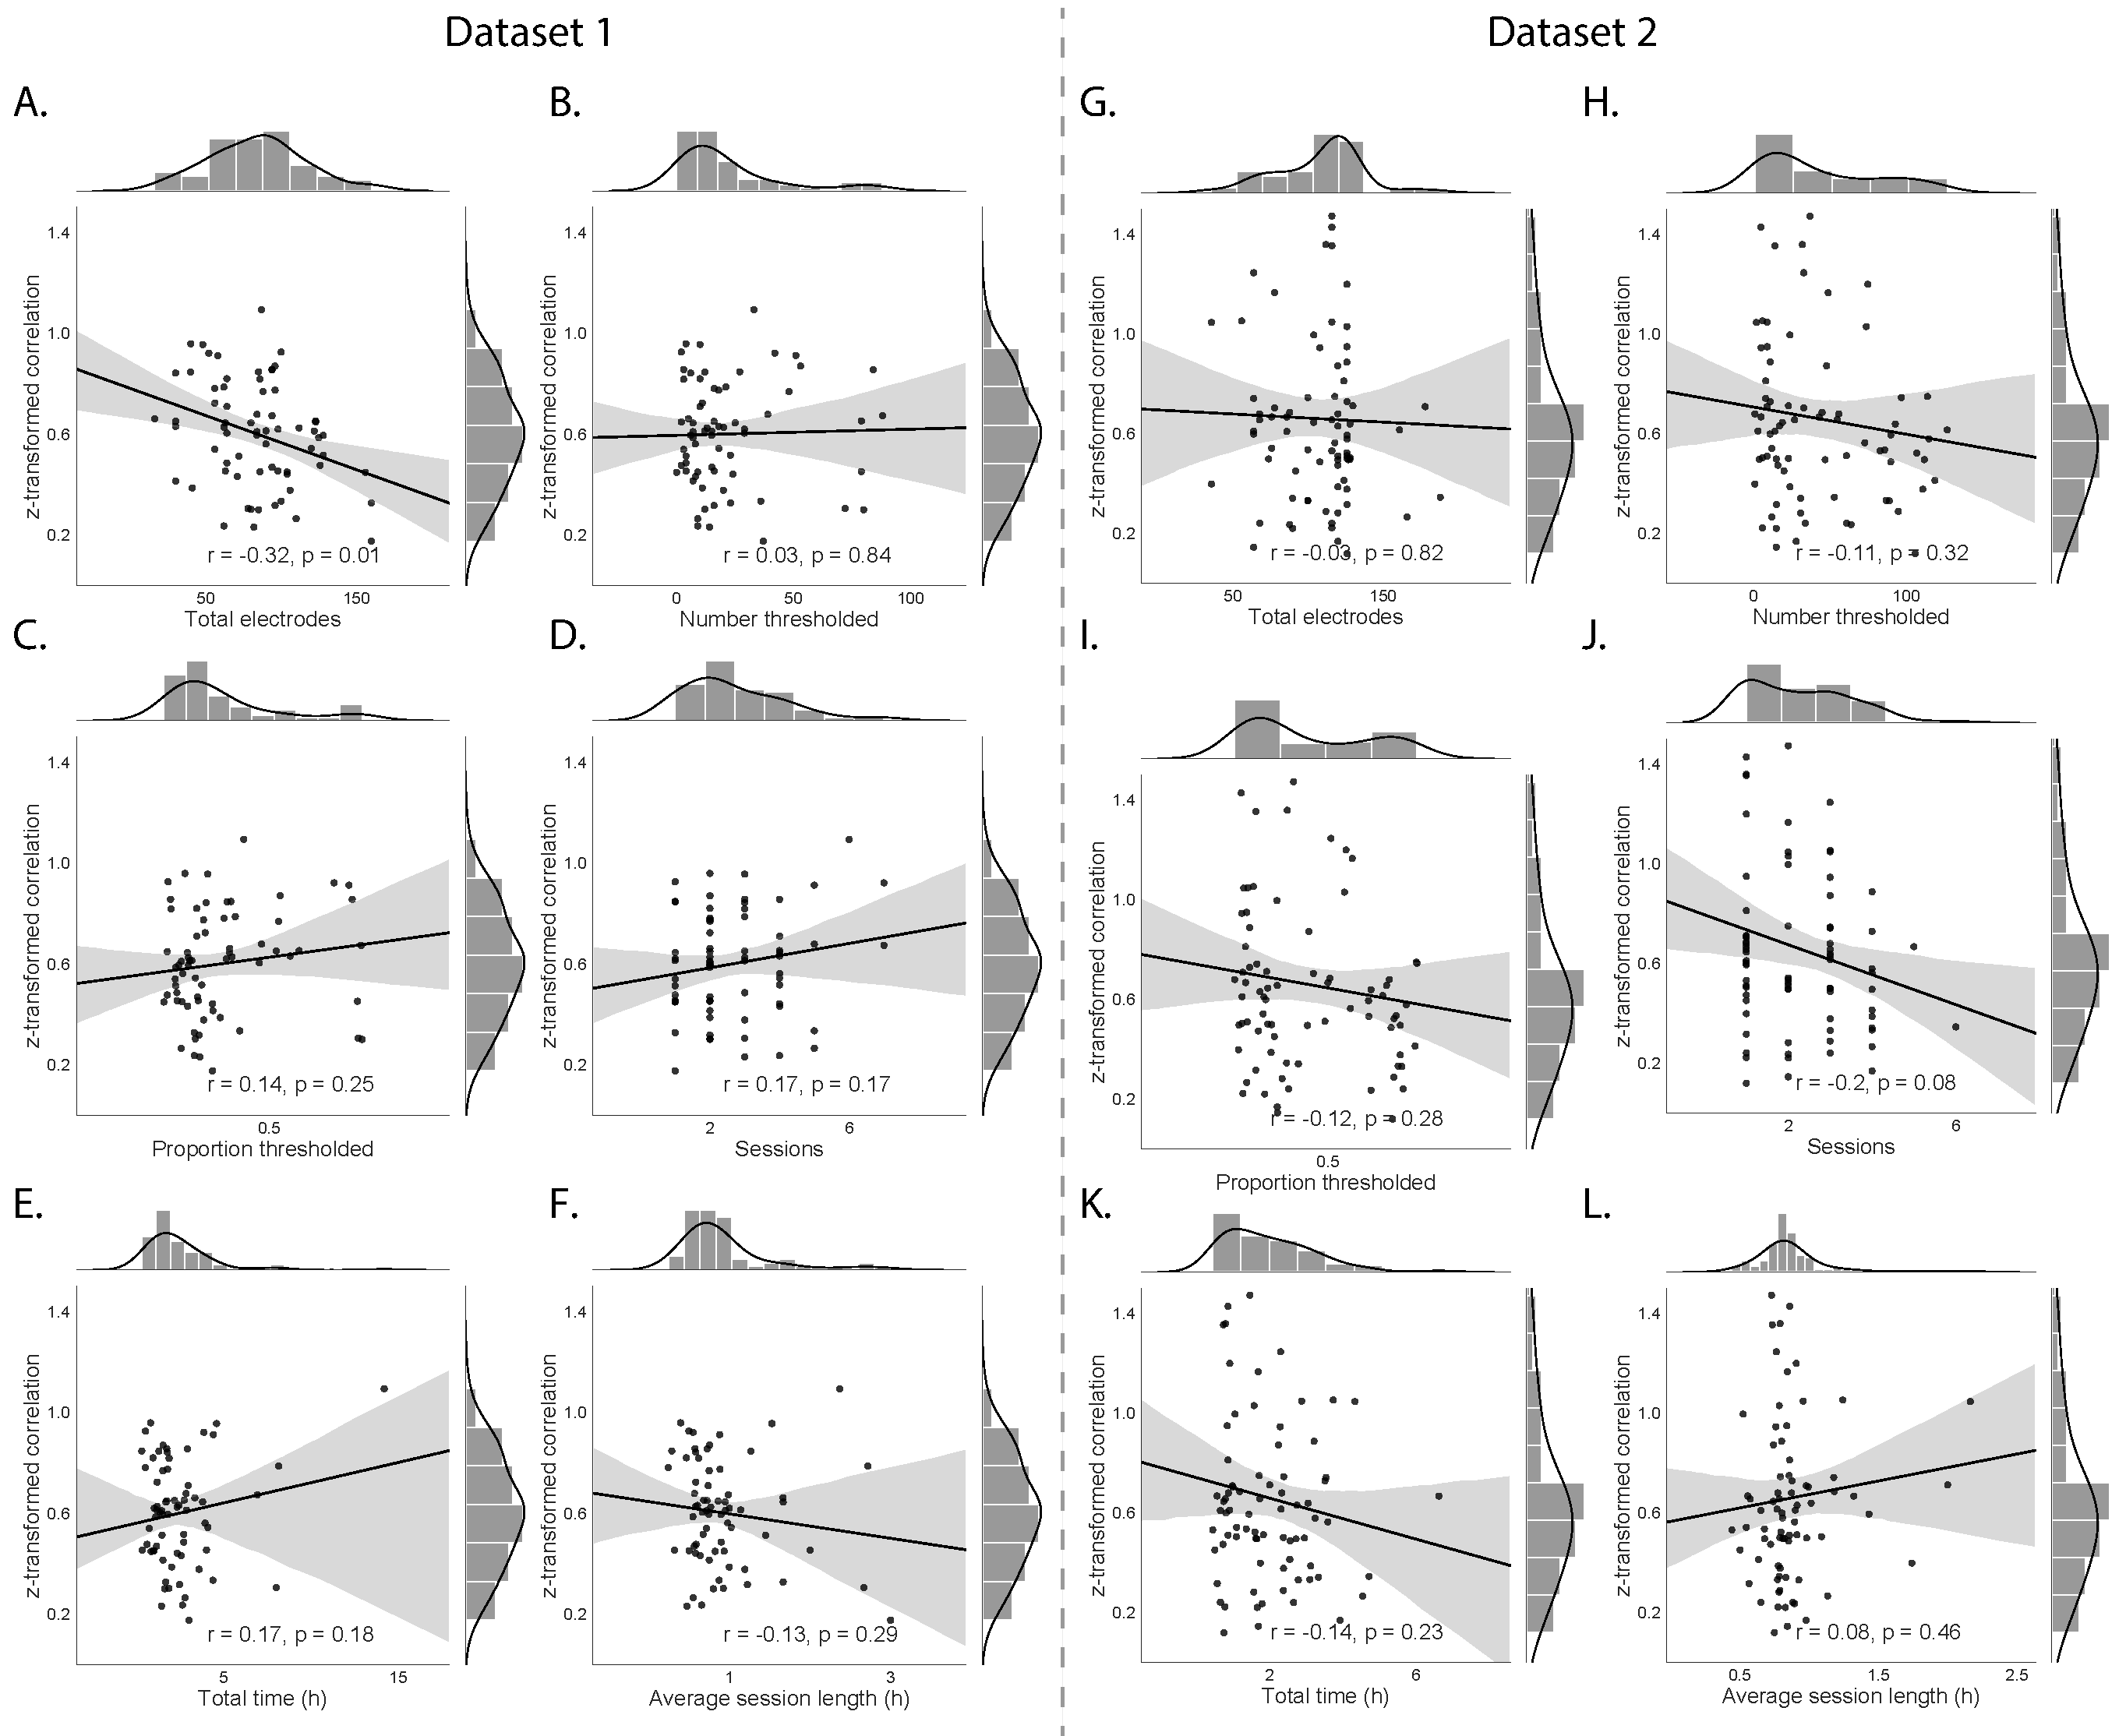
\includegraphics[width=\textwidth]{figs/supplemental_4}
\caption{\textbf{Reconstruction accuracy predicted by data
    features for each dataset.} \textbf{A.--F.  Features from Dataset
    1.}  Features include: (\textbf{A.}) number of electrodes,
  (\textbf{B.}) proportion thresholded, (\textbf{C.}), total recording
  time, (\textbf{D.}) number thresholded, (\textbf{E.}) number of
  sessions, and (\textbf{F.}) average session length.  The histograms
  report the distributions of the z-transformed correlation
  coefficients and the associated data feature.
  \textbf{G.--L. Features from Dataset 2.}  Analogous format to Panels
  A--F.}
\label{fig:supplemental_4}
\end{figure}


\begin{figure}[ptb]
\centering
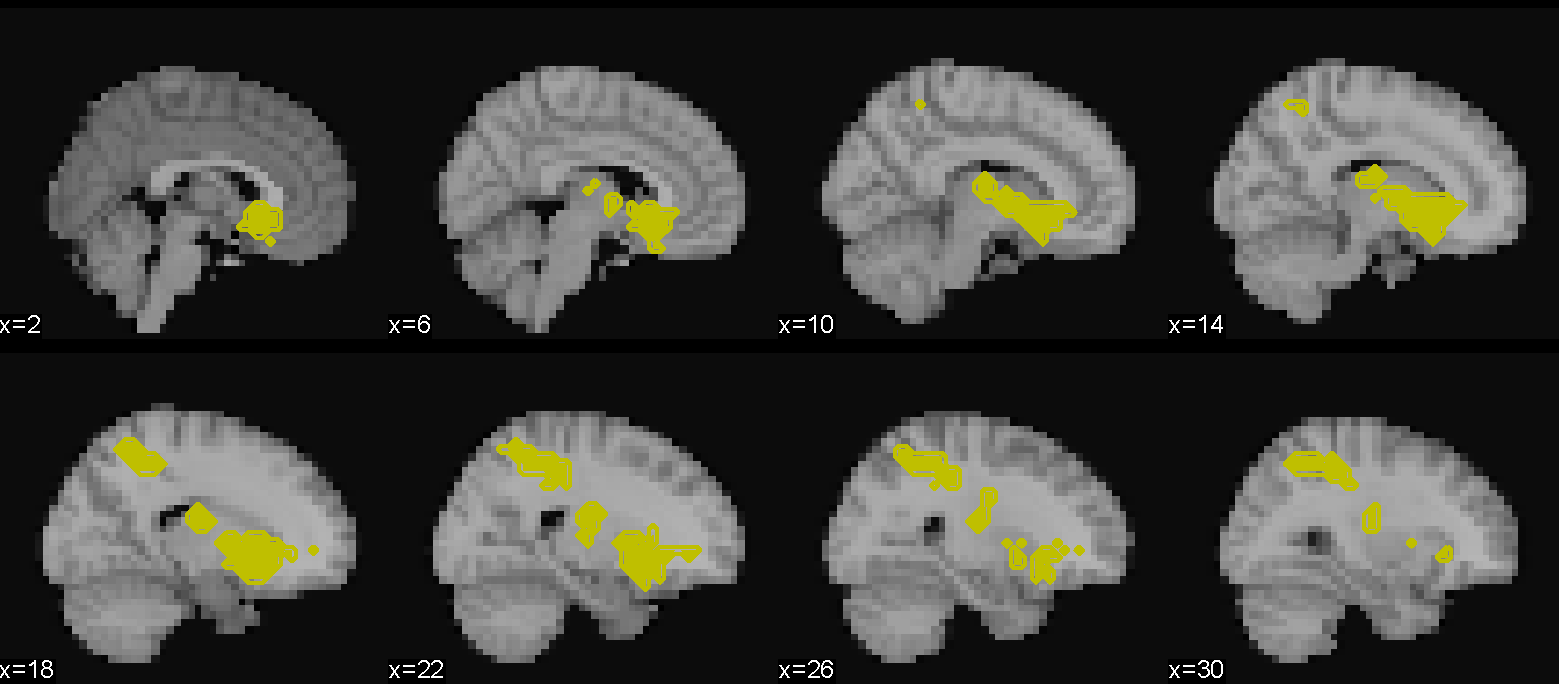
\includegraphics[width=\textwidth]{figs/supplemental_5}
\caption{\textbf{ Top 10\% most informative voxels.}
 Voxels in yellow indicate the intersections between
    the top 10\% most informative voxels in each brain map from Figure
    5, indicated by the white contours.}
\label{fig:supplemental_5}
\end{figure}


% \newpage
% \renewcommand{\refname}{Supplemental references}
% \bibliography{memlab}


\end{document}